\documentclass[tikz,border=12pt]{standalone}
\usepackage[utf8]{inputenc}\usepackage[T1]{fontenc}\usepackage{tikz}
\usetikzlibrary{arrows.meta,positioning,shadows.blur}
\definecolor{greenFill}{HTML}{E8F5E9}\definecolor{greenStroke}{HTML}{43A047}
\definecolor{coreFill}{HTML}{E1F5FE}\definecolor{coreStroke}{HTML}{0277BD}
\definecolor{optFill}{HTML}{FCE4EC}\definecolor{optStroke}{HTML}{D81B60}
\definecolor{memFill}{HTML}{FFF3E0}\definecolor{memStroke}{HTML}{EF8C00}
\begin{document}
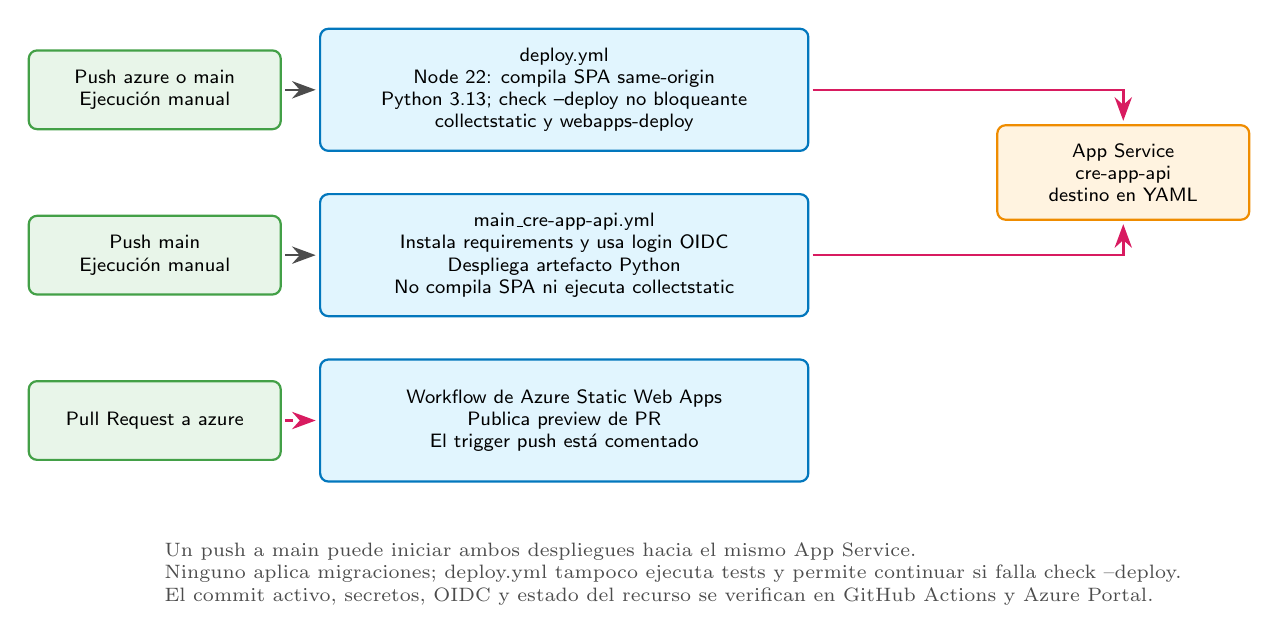
\begin{tikzpicture}[
  font=\sffamily\scriptsize,>={Stealth[length=3mm,width=2.2mm]},
  trigger/.style={rectangle,rounded corners=3pt,draw=greenStroke,thick,fill=greenFill,minimum width=3.2cm,minimum height=1.0cm,align=center},
  job/.style={rectangle,rounded corners=3pt,draw=coreStroke,thick,fill=coreFill,minimum width=6.2cm,minimum height=1.55cm,align=center},
  target/.style={rectangle,rounded corners=3pt,draw=memStroke,thick,fill=memFill,minimum width=3.2cm,minimum height=1.2cm,align=center},
  edge/.style={->,line width=.9pt,draw=black!70,shorten >=1.2pt,shorten <=1.2pt}, conflict/.style={->,line width=.9pt,draw=optStroke,shorten >=1.2pt,shorten <=1.2pt}, optional/.style={->,line width=.9pt,dashed,draw=optStroke,shorten >=1.2pt,shorten <=1.2pt}
]
% Three independent workflows are aligned in rows; only the two App Service pipelines converge.
\node[trigger] (deploytrigger) at (0,2.0) {Push azure o main\\Ejecución manual};
\node[job] (deploy) at (5.2,2.0) {deploy.yml\\Node 22: compila SPA same-origin\\Python 3.13; check --deploy no bloqueante\\collectstatic y webapps-deploy};
\node[trigger] (maintrigger) at (0,-0.1) {Push main\\Ejecución manual};
\node[job] (mainflow) at (5.2,-0.1) {main\_cre-app-api.yml\\Instala requirements y usa login OIDC\\Despliega artefacto Python\\No compila SPA ni ejecuta collectstatic};
\node[trigger] (prtrigger) at (0,-2.2) {Pull Request a azure};
\node[job] (swa) at (5.2,-2.2) {Workflow de Azure Static Web Apps\\Publica preview de PR\\El trigger push está comentado};
\node[target] (app) at (12.3,0.95) {App Service\\cre-app-api\\destino en YAML};
\draw[edge] (deploytrigger.east) -- (deploy.west);
\draw[edge] (maintrigger.east) -- (mainflow.west);
\draw[optional] (prtrigger.east) -- (swa.west);
\draw[conflict] (deploy.east) -| (app.north);
\draw[conflict] (mainflow.east) -| (app.south);
\node[font=\scriptsize,text=black!70,align=left,anchor=west] at (0,-4.15)
 {Un push a main puede iniciar ambos despliegues hacia el mismo App Service.\\
  Ninguno aplica migraciones; deploy.yml tampoco ejecuta tests y permite continuar si falla check --deploy.\\
  El commit activo, secretos, OIDC y estado del recurso se verifican en GitHub Actions y Azure Portal.};
\end{tikzpicture}
\end{document}
